\documentclass{VUMIFPSkursinis}
\usepackage{algorithmicx}
\usepackage{algorithm}
\usepackage{algpseudocode}
\usepackage{amsfonts}
\usepackage{amsmath}
\usepackage{bm}
\usepackage{caption}
\usepackage{color}
\usepackage{float}
\usepackage{graphicx}
\usepackage{listings}
\usepackage{subfig}
\usepackage{wrapfig}
\usepackage{sectsty}

\usepackage{enumitem}
%PAKEISTA, tarpai tarp sąrašo elementų
\setitemize{noitemsep,topsep=0pt,parsep=0pt,partopsep=0pt}
\setenumerate{noitemsep,topsep=0pt,parsep=0pt,partopsep=0pt}
\allsectionsfont{\centering}
% Titulinio aprašas
\university{Vilniaus universitetas}
\faculty{Matematikos ir informatikos fakultetas}
\department{Programų sistemų katedra}
\papertype{Programų sistemų inžinerijos III laboratorinis darbas}
\title{Socialinis Vilniaus universiteto tinklalapis}
\titleineng{SocialVU}
\status{2 kurso 4 grupės studentai}
\author{Andrejus Voitovas}
\secondauthor{Eglė Puodžiūnaitė}
\thirdauthor{Kasparas Kralikas}
\fourthauthor{Ieva Vizgirdaitė} % Pridėti antrą autorių
\supervisor{asist. dr. Vytautas Valaitis}
\date{Vilnius – \the\year}

% Nustatymai
% \setmainfont{Palemonas}   % Pakeisti teksto šriftą į Palemonas (turi būti įdiegtas sistemoje)
\bibliography{bibliografija}

\begin{document}
% PAKEISTA
\maketitle
\cleardoublepage\pagenumbering{arabic}
\setcounter{page}{2}
\sectionnonum{ANOTACIJA}
Šiame dokumente pateikiama dalykinės srities analizė. Išorinėje verslo proceso analizėje identifikuojamos pagrindinės grėsmės ir galimybės. Vidinėje verslo proceso analizėje nustatomos verslo stiprybės ir silpnybės, kylančios iš paties verslo proceso. Be to dokumente pateikiamos verslo tobulinimo strategijos, nagrinėjamos galimybės įgyvendinti sistemą tiek techniniu tiek ir ekonominiu požiūriu.\\
Rašant šį dokumentą buvo naudojamasi:
\begin{enumerate}
	\item dr. Vytauto Valaičio internetinis puslapiu (https://klevas.mif.vu.lt/~valaitis/) 
	\item doc., dr. Karolio Petrausko iternetiniu puslapiu (http://klevas.mif.vu.lt/~karolis/) 
	\item https://www.magicdraw.com/files/manuals/MagicDraw Tutorials.pdf
	\item Latex programa ir jau sukurtais šablonais
\end{enumerate}
\newpage
%TURINYS
\tableofcontents

\sectionnonum{ĮVADAS}
PATAISYT!!!
Šio dokumento tikslas - sukurti socialinio tinklalapio prototipą, kurį įgyvendinus būtų palengvinta universiteto bendruomenės komunikaciją.\\
\textbf{Temos aktualumas} \\
Šiuo metu studentams dėstytojų skelbiama informacija yra išbarstyta internete, kurią surasti užima galybes laiko. Yra atskiras universiteto naujienų puslapis, kiekvienas dėstytojas turi savo asmeninį tinklalapį, atskiras elektroninis paštas. Tiek dėstytojui pasiekti studentus, tiek studentui dėstytoją yra komplikuota ir nepatogu.\\
\textbf{Dalykinė sritis}\\
Socialinis Vilniaus Universiteto tinklapis.\\
 \textbf{Probleminė sritis}\\
Socialinis Vilniaus Universiteto tinklapis suteiktų galimybę greitai ir paprastai pasiekti šio universiteto dėstytojų puslapius, informaciją juose, susisiekti sus pačiais dėstytojais. Pagrindinis tinklalapio išskirtinumas - greitai ir patogiai pasiekiama informacija, viskas vienoje vietoje. Itin patogus valdymas dėstytojams.\\
 \textbf{Darbo pagrindas} \\ 
Dokumentas parengtas kaip Programų sistemų inžinerijos III laboratorinis darbas.
\newpage
\sectionnonum{VERSLO PROCESO APRAŠAS}
KASPARAS
\newpage
\section{IŠORINĖ VERSLO PROCESO ANALIZĖ}
Išorinė analizės metu išsiaiškinami ištekliai
reikalingi pradėti verslą, išryškinamos kuriamo verslo grėsmės ir
problemos, kuriami tinklalapio teikiami rezultatai ir išanalizuojama rinkoje esanti situacija. Nustačius rinkoje esančius ir potencialius konkurentus išanalizuojamos
neišnaudotos galimybės bei įvertinama situacija.

\ref{ieigos}, \ref{iseigos}, \ref{ivaizdis} ir \ref{reguliavimas} lentelėse pateikiami įeigos, išeigos, reguliavimo ir įvaizdžio svarbiausi vertinimo kriteriai,
jų matavimo vienetai. Nustatoma kritinė vertė, esama vertė ir siekiama vertė. Tai padeda
nustatyti, ar tam tikras vertinimo kriterijus atitinka normas.
\subsection{Įeigos}
\begin{enumerate}
	\item Studentai
	\item Dėstytojai
	\item Administratorius
	\item Duomenų bazė
	\item Serveris
\end{enumerate}
\begin{table}[H]
	\centering
	\caption{Įeigos}
	\resizebox{\textwidth}{!}{\begin{tabular}{|c|c|c|c|} \hline
			Vertinimo kriterijus & Mertinimo matas & Siekiama vertė & Kritinė vertė \\
			\hline
			Studentai & Kiekis studentų, naudojančių socialVU tinklalapį & 21281 & 10000 \\
			\hline
			Dėstytojai & Kiekis dėstytojų, naudojančių socialVU tinklalapį & 2890 & 1500 \\
			\hline
			Administratorius & Pašalintų naudotojų skaičius per
			mėnesį & 0 & 30 \\
			\hline
			Duomenų bazė & Talpa GB & 50 & 10 \\
			\hline
			Serveris & Vidutinis užklausos apdorojimo laikas sekundėmis & 1 & 5 \\
			\hline
	\end{tabular}}
	\label{ieigos}
\end{table}
\subsection{Išeigos}
\begin{enumerate}
	\item Studentai, radę visą reikiamą informaciją
	\item Dėstytojai, pateikę visą norimą informaciją
\end{enumerate}
\begin{table}[H]
	\centering
	\caption{Išeigos}
	{\begin{tabular}{|c|c|c|c|} \hline
			Vertinimo kriterijus & Mertinimo matas & Siekiama vertė & Kritinė vertė \\
			\hline
			Studentai, radę visą reikiamą informaciją & Kiekis per mėnesį \% & 100 & 50 \\
			\hline
			Dėstytojai, pateikę visą norimą informaciją & Kiekis per mėnesį \% & 100 & 50 \\
			\hline
	\end{tabular}}
	\label{iseigos}
\end{table}
	\subsection{Įvaizdis}
\begin{enumerate}
	\item Dėstytojų bei studentų atsiliepimai
	\item Sistemos žinomumas
\end{enumerate}
\begin{table}[H]
	\centering
	\caption{Įvaizdis}
	{\begin{tabular}{|c|c|c|c|} \hline
			Vertinimo kriterijus & Mertinimo matas & Siekiama vertė & Kritinė vertė \\
			\hline
			Dėstytojų bei studentų atsiliepimai & Teigiamų atsiliepimų \% nuo visų atsiliepimų & 90 & 50 \\
			\hline
			Sistemos žinomumas & Vilniaus universiteto studentų \% žinančių šį tinklalapį & 100 & 50 \\
			\hline
	\end{tabular}}
	\label{ivaizdis}
\end{table}
	\subsection{Reguliavimas}
\begin{enumerate}
	\item Asmens duomenų teisinės apsaugos įstatymas
	\item Darbo kodeksas
\end{enumerate}
\begin{table}[H]
	\centering
	\caption{Įvaizdis}
	{\begin{tabular}{|c|c|c|c|} \hline
			Vertinimo kriterijus & Mertinimo matas & Siekiama vertė & Kritinė vertė \\
			\hline
			Asmens duomenų teisinės apsaugos įstatymas & Pažeidimų skaičius & 0 & 0 \\
			\hline
			Darbo kodeksas & Viršytas darbo laikas (kartais per metus) & 0 & 0 \\
			\hline
	\end{tabular}}
	\label{reguliavimas}
\end{table}
\subsection{Grėsmės}
Kuriamas verslas yra priklausomas nuo dviejų pagrindinių įvesčių - dėstytojų ir studentų. Jų skaičius ir aktyvumas lemia kuriamos programos sėkmę. Rinkoje jau egzistuoja nemažai socialinių tinklų, kuriuos naudoja dauguma studentų (Facebook, Instagram, Linkedin, Twitter ir t.t.) be to dauguma dėstytojų yra ipratę skelbti visą informaciją savo sukurtuose puslapiuose arba bando integruoti informaciją į Vilniaus universiteto virtualią mokymosi aplinką, todėl konkurencija yra gana didelė. Kuo daugiau dėstytojų pradės naudoti mūsų sukurtą platformą, tuo daugiau studentų taip pat privalės naudoti šį tinklalapį, nes tik ten galės rasti jiems reikiamą informaciją. Sėkmingam kuriamo verslo proceso egzistavimui turi įtakos reitingų ir atsiliepimų skaičius bei kokybė, tačiau visų pirma reikia užtikrinti, jog dauguma studentų bei dėstytojų išbandytų mūsų sukurtą sistemą bei ją įvertintų.
\subsection{Neišnaudotos galimybės}
Rinkoje jau egzistuojančios Vilniaus universiteto platformos turi trūkumų (dauguma dėstytojų skelbia informaciją skirtinguose puslapiuose, todėl studentams sunku juos surasti, ne visada yra galimybė susisiekti su dėstytojais, dauguma konspektų nėra lengvai pasiekiami visiems studentams), todėl kuriama sistema gali juos išnaudoti ir pasiūlyti studentams visą reikiamą informaciją rasti vienoje vietoje. Sistema suteiks galimybę išsiųsti laišką dėstytojui bei rasti visą paskelbtą dėstytojo informaciją vienoje vietoje, studentai galės matyti naujausią informaciją bei terminus iki kada turi atlikti tam tikras užduotis. Be to vienoje vietoje galės rasti visus reikiamus konpektus bei pasidalinti turimais konspektais su kitais studentais ir taip padėti mokytis kitiems.
\newpage
\newpage
\section{VIDINĖ VERSLO PROCESO ANALIZĖ}
Toliau pateikiama keliais aspektais atlikta vidinė verslo proceso analizė, kuria siekiama
nustatyti nagrinėjamo verslo stiprybes ir silpnybes, kylančias iš verslo proceso.
\subsection{Dalykinės srities statinė stukrtūra}
 Toliau pateikiama dalykinės srities statinės struktūros UML diagrama. Joje matomos pagrindinės esybės bei jų tarpusavio sąveika. Klientai yra dviejų tipų: studentai, dėstytojai ir administratoriai (dėstytojai bei administratoriai skiriasi turinio redagavimo teisėmis). Studentams, administratoriams ir dėstytojams registruotis nereikia, nes visa vartotojų duomenų bazė bus imama iš bendros VU vartotojų duomenų bazės. Vartotojui tereikia autentifikuoti save - tokiu būdu, priklausomai nuo užimamų pareigų, jam bus suteiktos teisės prie numatyto turinio. Studentai gali tik skaityti tokius puslapius kaip "Dėstytojai", "Naujienos", "Renginiai", "D.U.K". Tuo tarpu dėstytojai skiltyje "Naujienos" gali parašyti naujieną. Be to, jiems suteikta prieiga prie jų profilio, kur turi teisę redaguoti savo asmeninį puslapį pagal mūsų sukurtą šabloną, siųsti bei gauti žinutes, pridėti organizuojamą renginį. Administratoriumi gali būti fakulteto paskirtas žmogus, atsakingas už tikslingo turinio formavimą vidiniame socialiniame tinkle arba VU Studento atstovybės narys, kuris turi teisę redaguoti visą turinį. Tačiau joks administratorius negali redaguoti dėstytojo sukurto turinio, nes taip numato mūsų kurtas produktas.\\

\begin{figure}[H]
\centering
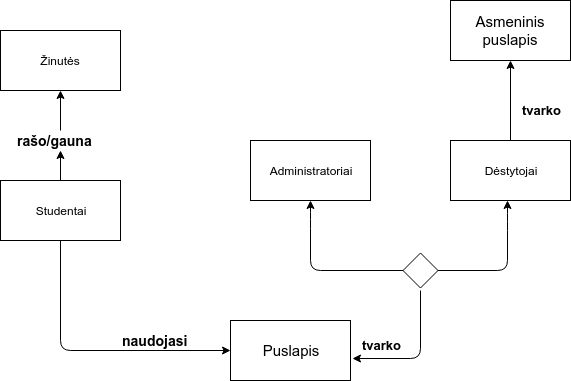
\includegraphics[width=\linewidth]{img/dalykine.png}
\label{fig:dalykine}
\caption{Dalykinė srities UML diagrama}
\end{figure}

SĄVOKOS: \\
Šiame skyriuje pateikiami specifiniai mūsų projekte naudotų žodžių paaiškinimai. \\
\textbf{Sistema} – fakulteto vidinis socialinis tinklas, dokumente vadinamas „SocialVU“. \\
\textbf{Studentas} – vartotojas, kuris turim ribotas galimybes turinio valdymo atžvilgiu.\\
\textbf{Dėstytojas} – vartotojas, kuris turi galimybę redaguoti visą socialinio tinklo turinį.\\
\textbf{Administratorius} – vartotojas, kuris turi galimybę redaguoti visą socialinio tinklo turinį, išskyrus dėstytojus.

\subsection{Užduotys}
\begin{figure}[H]
\centering
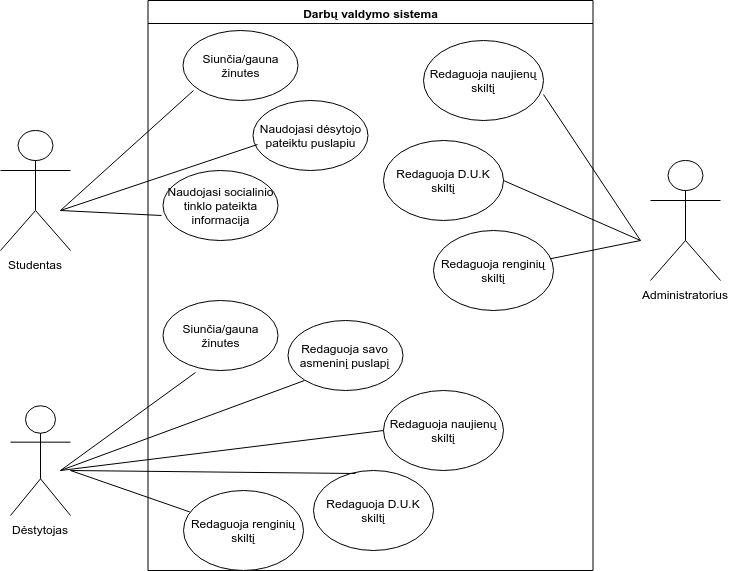
\includegraphics[width=\linewidth]{img/DVS.png}
\caption{Užduočių veiklos UML diagrama}
\label{fig:dvs}
\end{figure}
\setlength{\parindent}{0pt}Užduočių sąrašas pagal \ref{fig:dvs} pav.:\\
\setlength{\parindent}{0pt}\textbf{Užduotis:} sukurti naujieną. \\
\textbf{Tikslas:} publikuoti naujieną, kuri būtų įdomi.\\
\textbf{Trigeris:} administratoriaus arba dėstytojo kuriama naujiena tituliniui. \\
\textbf{Prioritetas:} aukštas. \\
\textbf{„Prieš” sąlygos:} naujiena bus skaitoma.\\
\textbf{Sėkmingos baigties „po” sąlyga:} naujiena perskaitoma ir įsisavinama nauja informacija. \\
\textbf{Nesėkmingos baigties sąlyga:} naujiena visiškai nėra skaitoma. \\
\textbf{Pirminis agentas:} administratorius. \\
\textbf{Antriniai agentai:} studentas. \\

\setlength{\parindent}{0pt}\textbf{Užduotis:} redaguoti puslapį. \\
\textbf{Tikslas:} redaguoti dėstytojo puslapį.\\
\textbf{Trigeris:} prisijungęs dėstytojas gali redaguoti puslapį. \\
\textbf{Prioritetas:} aukštas. \\
\textbf{„Prieš” sąlygos:} dėstytojas patogiai talpina informaciją.\\
\textbf{Sėkmingos baigties „po” sąlyga:} dėstytojo informacija sudėliota pagal šabloną ir patogi naudojimuisi. \\
\textbf{Nesėkmingos baigties sąlyga:} dėstytojas nesudaro savo puslapio. \\
\textbf{Pirminis agentas:} dėstytojas. \\
\textbf{Antriniai agentai:} studentas. \\

\setlength{\parindent}{0pt}\textbf{Užduotis:} sukurti renginį. \\
\textbf{Tikslas:} publikuoti renginį, kuris būtų naudingas.\\
\textbf{Trigeris:} administratoriaus arba dėstytojo sukurtas renginys atsiranda puslapyje. \\
\textbf{Prioritetas:} aukštas. \\
\textbf{„Prieš” sąlygos:} renginį aplankys daug žmonių.\\
\textbf{Sėkmingos baigties „po” sąlyga:} renginys pateisino savo lūkesčius. \\
\textbf{Nesėkmingos baigties sąlyga:} apie renginį studentai sužinojo ne iš socialinio tinklo. \\
\textbf{Pirminis agentas:} administratorius. \\
\textbf{Antriniai agentai:} studentas. \\


\setlength{\parindent}{0pt}\textbf{Užduotis:} parašyti žinutę. \\
\textbf{Tikslas:} parašyti žinutę tiesiai vartotojui.\\
\textbf{Trigeris:} studentas, paspaudęs ant dėstytojo, gali parašyti jam žinutę. \\
\textbf{Prioritetas:} aukštas. \\
\textbf{„Prieš” sąlygos:} vartotojas gaus žinutę.\\
\textbf{Sėkmingos baigties „po” sąlyga:} vartotojai patogiai komunikuos tarpusavy. \\
\textbf{Nesėkmingos baigties sąlyga:} žinutė liks neperskaityta. \\
\textbf{Pirminis agentas:} studentas. \\
\textbf{Antriniai agentai:} administratorius.\\

\setlength{\parindent}{0pt} \textbf{Užduotis:} apsilankyti asmeniniame puslapyje. \\
\textbf{Tikslas:} pasiekti dėsytotojo asmeninį puslapį.\\
\textbf{Trigeris:} studentų apsilankymas dėstytojų profilyje. \\
\textbf{Prioritetas:} aukštas. \\
\textbf{„Prieš” sąlygos:} vartotojai lankysis dėstytojų puslapiuose per socialinį tinklą.\\
\textbf{Sėkmingos baigties „po” sąlyga:} vartotojams bus patogu pasiekti puslapį ir sužinoti informaciją. \\
\textbf{Nesėkmingos baigties sąlyga:} vartotojai toliau ieškos puslapių naudojantis "Google". \\
\textbf{Pirminis agentas:} studentas. \\
\textbf{Antriniai agentai:} administratorius.

\subsection{Užduočių vykdymo scenarijai}
\ref{fig:klasiu} pav. paveikslėlyje pavaizduota esybių diagrama. Pateikiamos pagrindinės dalykinės srities esybės, pavaizduoti ryšiai tarp jų.
\begin{figure}[H]
\centering
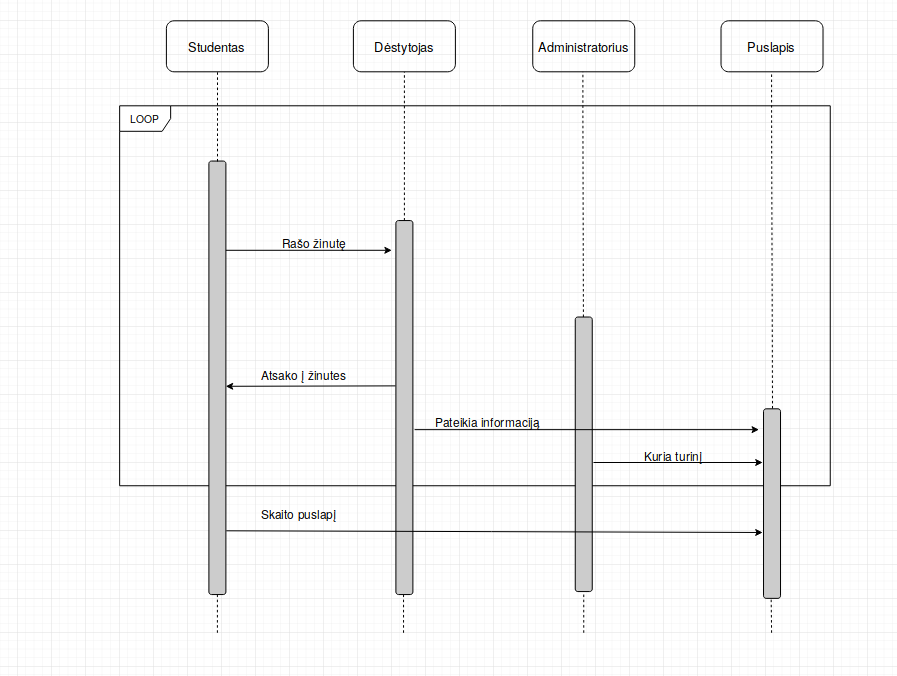
\includegraphics[width=\linewidth]{img/bendra-uml.png}
\caption{Klasių diagrama}
\label{fig:klasiu}
\end{figure}
\ref{fig:klasiu} pav. vaizuduojamas socialinio tinklo naudojimosi modelis. Studentas gali rašyti dėstytojui žinutę, o dėstytojas jam gali atsakyti. Taip pat studentas skaito puslapį, kurį pats dėstytojas ir sukūrė. Administratorius kuria turinį, į kurį įeina: renginiai, naujienos, D.U.K.
\subsection{Dalykinės srities dinaminė struktūra}
Studentas:
\begin{figure}[H]
\centering
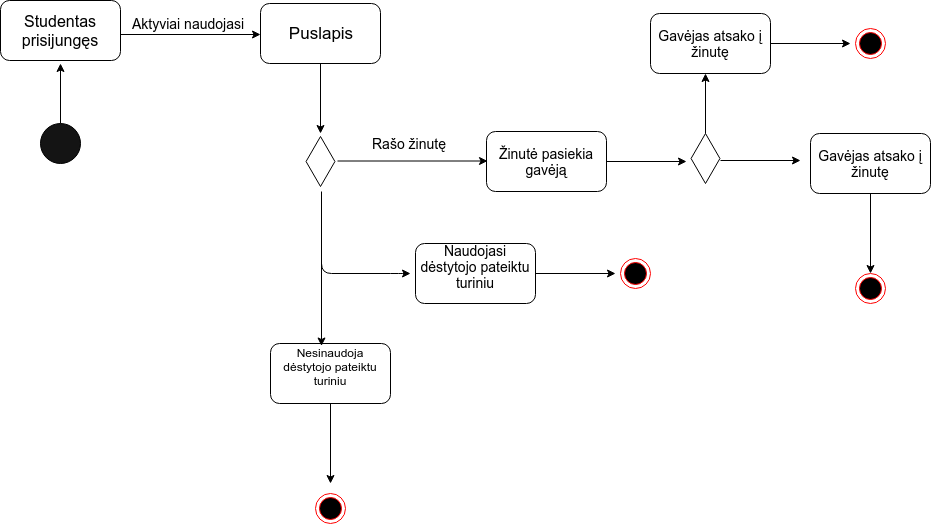
\includegraphics[width=\linewidth]{img/studentas.png}
\caption{Studento UML klasių diagrama}
\label{fig:studentu}
\end{figure}
\ref{fig:studentu} pav. Prisijungęs studentas turi galimybę matyti bendrą turinį. Vėliau gali parašyti žinutę dėstytojui arba naudojasi dėstytojo pateiktu turiniu. Jie tarpusavyje gali komunikuoti socialinio tinklo pagalba, nenaudojant trečiųjų šalių servisų.\\
Dėstytojas: \\
\begin{figure}[H]
\centering
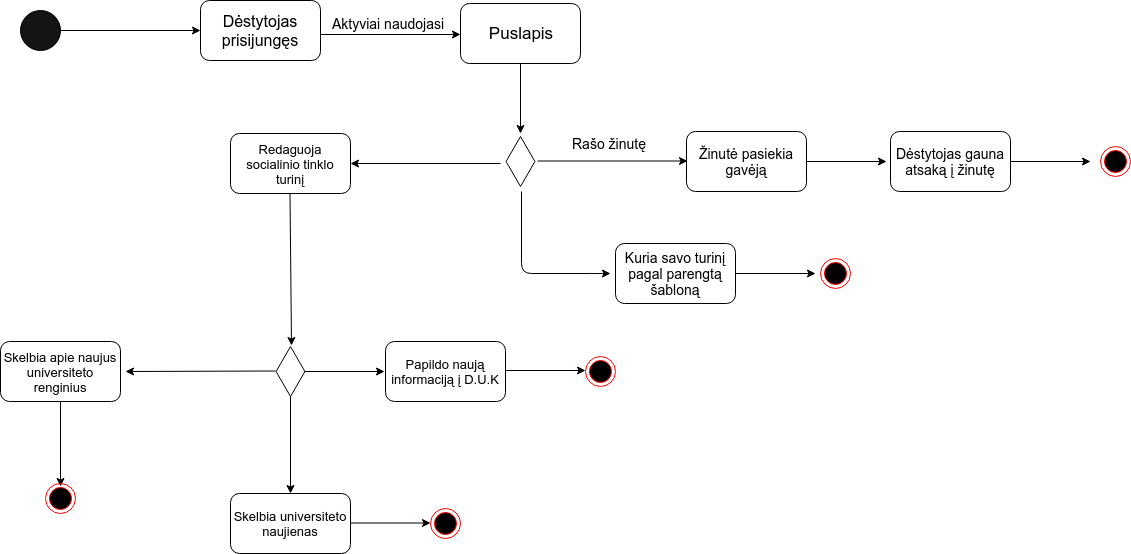
\includegraphics[width=\linewidth]{img/destytojas.png}
\caption{Dėstytojo UML klasių diagrama}
\label{fig:destytoju}
\end{figure}
\ref{fig:destytoju} pav. Prisijungęs dėstytojas turi galimybę redaguoti savo puslapio turinį, pagal iš anksto paruoštą šabloną. Dar turi galimybę rašyti bei atsakyti į studentų gautas žinutes. Naujienų rašymas, renginių kūrimas, D.U.K skilties papildymas irgi įeina į aukščiau aprašomo vartotojo galimybes.\\
Administratorius: \\
\begin{figure}[H]
\centering
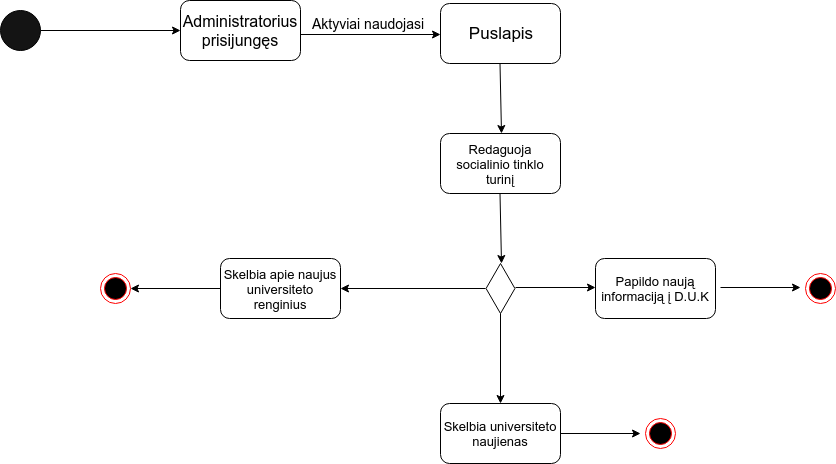
\includegraphics[width=\linewidth]{img/administratorius.png}
\caption{Administratoriaus UML klasių diagrama}
\label{fig:administratoriu}
\end{figure}
\ref{fig:administratoriu} pav. Prisijungęs administratorius, tai žmogus, kuris atsakingas už bendrą socialinio tinklo turinį, į kurį neįeina dėstytojų puslapių redagavimas. Administratorius gali kurti bei redaguoti tik naujienų, D.U.K ir renginių skiltis.\\

\newpage
\section{ĮGYVENDINAMUMO IR NAUDOS ANALIZĖ}
Šiame skyriuje pateikiama informacija, kuri padeda nustatyti, ar darbų valdymo sistemą
įmanoma sukurti, kokią konkrečią naudą ji duos, kokios problemos gali kilti ir kaip jos bus sprendžiamos.

\subsection{Operacinis įgyvendinamumas}
Šiame skyriuje pateikiami galimi trukdžiai, kurie gali kilti naudantis sistema, bei pateikiami
galimi jų sprendimo būdai.
\bigskip

\textbf{Problema:}

\textbf{Sprendimo būdas:}

\bigskip

\textbf{Problema:}

\textbf{Sprendimo būdas:}

\bigskip

\textbf{Problema:}

\textbf{Sprendimo būdas:}

\subsection{Techninis įgyvendinamumas}
Lorem ipsum dolor sit amet, consectetur adipiscing elit. Morbi id mauris eu lacus porttitor euismod. Nunc in turpis in magna hendrerit fermentum. Nam porta at lorem eget faucibus. Vestibulum vitae luctus lectus. Nunc aliquet nibh arcu. Pellentesque at convallis odio, in accumsan felis. Praesent pulvinar in erat et porttitor. Aliquam viverra lobortis orci, vitae porta neque rhoncus sagittis. Phasellus et faucibus est. Duis in sodales massa. Fusce id finibus nisl. Curabitur justo nisi, sodales eu lobortis luctus, porttitor sed nisl. Donec vel leo in nisl consectetur vestibulum id in libero.

\subsection{Ekonominis įgyvendinamumas}

\textbf{Išlaidos}

\begin{table}[H]
	\centering
	\caption{Išlaidos reikalingos sistemos sukūrimui ir palaikymui}
    {\begin{tabular}{|c|c|c|c|} \hline
			Išlaidos & Kaina  \\
			\hline
			Sistemos sukūrimas & 5€ \\
			\hline
			Serverio nuoma & 12€ metams \\
			\hline
	\end{tabular}}
\end{table}
\newpage

\section{SISTEMOS NAUDOJIMO SCENARIJUS}
Šiame skyriuje aprašomas socialinio tinklalapio naudojimo scenarijus
\subsection{Scenarijus}
Šiame skyriuje pateikiami pagrindinių funkcijų modeliai, kurie parodo, kaip pagrindiniai sistemos agentai, šiuo atveju studentai, dėstytojai ir administratoriai, naudosis sistema. Tam naudojamos UML sekų diagramos.
\subsubsection{Užduoties registruotis modelis}
\begin{figure}[H]
\centering
\includegraphics[width=\linewidth]{img/uzdRegistruotis.png}
\caption{Užduoties registruotis modelis}
\label{fig:registruotis}
\end{figure}
\textbf{Užduotis: } užregistruoti naują naudotoją.\\
\textbf{Verslo sistema: }\\
\textbf{Tikslas: } pradėti naudotis socialiniu tinklalapiu.\\
\textbf{Pirminis agentas: } naudotojas.\\
\textbf{"Prieš" sąlyga: } naudotojas atsidaręs socialinį tinklalapį.\\
\textbf{"Po" sąlyga: } naudotojas gali siųsti žinutes kitiems naudotojams, matyti tik naudotojams skirtą informaciją.\\
\textbf{Scenarijus: } naudotojas, atsidaręs socialinį tinklalapį ir užėjęs į registracijos formą, turi įvesti savo duomenis: vardą, pavardę, e. pašto adresą, pasirinkti studentas ar dėstytojas. Pasirinkus dėstytoją dar įvesti specialų identifikacijos raktą gautą iš administratoriaus. Naudotojas registracijos formoje taip pat turi pažymėti, kad sutinka su tinklalapio sąlygomis. Jeigu įvesti duomenys neatitinka formato arba toks klientas jau yra registruotas, naudotojui parodomas klaidos praneši- mas. Jeigu registracija sėkminga, naudotojui yra pranešama apie sėkmingą registraciją ir jis yra nukreipiamas į pagrindinį sistemos puslapį.\\
\subsubsection{Užduoties įrašyti naujieną modelis}
\begin{figure}[H]
\centering
\includegraphics[width=\linewidth]{img/uzdNaujiena.png}
\caption{Užduoties įrašyti naujieną modelis}
\label{fig:rnaujiena}
\end{figure}
\textbf{Užduotis: } Įrašyti naujieną\\
\textbf{Verslo sistema: }\\
\textbf{Tikslas: } paskelbti aktualią naujieną.\\
\textbf{Pirminis agentas: } dėstytojas.\\
\textbf{"Prieš" sąlyga: } naudotojas yra prisijungęs tinklalapyje, dėstytojo aplinkoje.\\
\textbf{"Po" sąlyga: } aktuali naujiena yra patalpinta tinklalapyje.\\
\textbf{Scenarijus: } naudotojas, prisijungęs kaip dėstytojas, pasirenka naujienos sukūrimo puslapį ir gražintoje formoje suveda norimą paskelbti informaciją bei pasirenka, kam ši naujiena yra skirta(studentams, dėstytojams, visiems). Jeigu naujiena neatitinka formato ar yra tuščia, sistema įspėja dėstytoją ir leidžia pakeisti duomenis. Jeigu duomenys atitinka formatą, dėstytojas yra informuojamas apie sėkmingą naujienos patalpinimą pagrindiniame puslapyje.
\subsubsection{Užduoties siųsti žinutę modelis}
\begin{figure}[H]
\centering
\includegraphics[width=\linewidth]{img/uzdSiustiZinute.png}
\caption{Užduoties siųsti žinutę modelis}
\label{fig:zinute}
\end{figure}
\textbf{Užduotis: } studentui išsiųsti žinutę dėstytojui\\
\textbf{Verslo sistema: }\\
\textbf{Tikslas: } studento išsiųsta žinutė pasiekia dėstytoją\\
\textbf{Pirminis agentas: } studentas\\
\textbf{"Prieš" sąlyga: } naudotojas yra prisijungęs tinklalapyje, studento aplinkoje.\\
\textbf{"Po" sąlyga: } studento žinutė yra išsiųsta\\
\textbf{Scenarijus: } naudotojas, prisijungęs kaip studentas, pasirenka puslapį siųsti žinutę. Gražintoje formoje pasirenka dėstytoją(us), kuriam(iem) ši žinutė yra skirta. Užpildo formoje prašomus duomenis (tema, žinutė), prisega failus, jeigu reikia. Jeigu žinutė neatitinka formato, sistema įspėja studentą ir leidžia pakeisti duomenis. Jeigu bandomų pridėti failų napvyko prisegti, studentas įspėjamas. Jeigu žinutė atitinka formatą ir failai sėkmingai prisegti, studentas informuojamas, jog žinutė išsiųsta sėkmingai.
\subsection{Sistemos teikiama nauda}
Šiame skyriuje nagrinėjamos užduotys, kurias gali atlikti naudotojai. Tam pavaizduoti naudojama UML užduočių diagrama, kurioje agentai yra mūsų sistemos naudotojai - studentai ir dėstytojai.
\begin{figure}[H]
\centering
\includegraphics[width=\linewidth]{img/socpslSistema.png}
\caption{Užduočių diagrama}
\label{fig:uzdDiagram}
\end{figure}
Sistemoje vykdomos pagrindinės užduotys: studentas gali peržiūrėti pasirinkto dėstytojo puslapius. Dėstytojams sudaroma galimybė pateikti aktualias naujienas, informaciją apie renginius, redaguoti savo asmeninius tinklalapius, kuriuose gali talpinti informaciją apie savo dėstomus dalykus bei kitą naudingą informaciją, kurią matys jų studentai. Tiek dėstytojai, tiek studentai gali gauti informaciją apie juos dominančius renginius, matyti aktualias naujienas, gauti bei siųsti žinutes.(\ref{fig:uzdDiagram} pav.).
\subsection{Esama būklė}
Šiuo metu visi komandos nariai turi asmeninius kompiuterius kuriais gali kurti ir testuoti sistemą. Nariai taip pat turi priėjimą prie Android ir iOS išmaniųjų telefonų, kurių prireiks tinklapio testavimui mobiliuose įrenginiuose. Grupė sudaryta iš keturių asmenų, kurie yra įgiję reikalingas žinias sistemos sukūrimui ir palaikymui.
\subsection{Priemonės scenarijui įgyvendinti}
Norint sukurti socialinį tinklalapį bus reikalinga:
\begin{enumerate}
	\item Domeno registracija
	\item Serveris
	\item SSL sertifikatas
\end{enumerate}
\end{document}
\sectionnonum{REZULTATAI}
